% Toy paper for the AI for Research seminar.
%
% Illustrative only. Filled in from the Stack Overflow Annual Developer
% Survey 2025. All numbers come from ../results_table.csv, produced by
% analysis/analysis.py. See ../README.md for the workflow.

\documentclass[11pt]{article}

\usepackage[a4paper, margin=2.5cm]{geometry}
\usepackage{amsmath}
\usepackage{graphicx}
\usepackage{booktabs}
\usepackage{hyperref}
\usepackage{natbib}
\usepackage{authblk}

\title{AI-tool adoption and self-reported job satisfaction among professional
software developers: a descriptive analysis of the Stack Overflow Annual
Developer Survey}

\author[1]{Author One}
\author[1]{Author Two}
\affil[1]{Universidade Cat\'olica Portuguesa}

\date{\today}

\begin{document}
\maketitle

\begin{abstract}
This is a descriptive study. Using the Stack Overflow Annual Developer
Survey 2025, we document the cross-sectional relationship between
professional developers' reported adoption of AI coding tools and their
reported job satisfaction, controlling for years of professional experience
and primary developer role. In an analysis sample of 24{,}318
professional developers with complete data, daily and occasional AI-tool
users report job satisfaction about $0.15$ points higher (on a $0$--$10$
scale) than non-users after adjustment, a difference that is statistically
distinguishable from zero ($p < 0.001$) but small in magnitude: the
specification explains only about $2\%$ of the variation in satisfaction.
We make no causal claim. The survey is observational, selection into it is
not random, and both AI-tool adoption and satisfaction are self-reported,
with no instrument for adoption and no longitudinal variation. We spell out
these limits in detail. This paper is a teaching artefact produced for a
seminar on AI for research; it is not intended for publication.
\end{abstract}

\section{Introduction}
AI coding assistants moved, in a short span, from novelty to default part
of many developers' daily workflow. A natural and frequently asked question
is whether developers who adopt these tools are, on average, more satisfied
with their jobs --- whether because the tools remove drudgery, or simply
because the kind of developer who adopts them differs in ways that also
relate to satisfaction. The Stack Overflow Annual Developer Survey, which
reaches tens of thousands of developers and asks about both AI-tool use and
job satisfaction, is a convenient place to look at this association
descriptively.

We emphasise at the outset that this is a descriptive exercise. We document
a correlation in a single cross-section of self-reported data; we do not
estimate the effect of AI-tool adoption on satisfaction, and nothing in our
design would license that interpretation. AI-tool adoption is a choice that
is plausibly correlated with developer ability, team culture, employer, and
even with satisfaction itself. We therefore report associations, flag the
threats to any causal reading prominently (Section~\ref{sec:limitations}),
and resist causal language throughout.

Our contribution is pedagogical rather than substantive. The paper is a
transparent, end-to-end worked example for a seminar on using AI tools in
the research workflow: a public dataset, a clearly stated descriptive
question, a small reproducible analysis, and an honest accounting of what
the data can and cannot support. The ``finding'' is incidental; the worked
example is the point.

\section{Data}
\label{sec:data}
We use the Stack Overflow Annual Developer Survey 2025
\citep{stackoverflow2025survey}, a large annual online survey of software
developers recruited primarily through Stack Overflow's own channels.
Participation is voluntary and unincentivised, so the sample is one of
convenience rather than a probability sample of any defined developer
population. The public release contains 49{,}191 responses. The data are
distributed under the Open Database License (ODbL) 1.0 and the Database
Contents License (DbCL) 1.0; we attribute Stack Overflow as the source as
those licenses require.

We restrict attention to respondents who identify as professional
developers (\texttt{MainBranch} $=$ ``I am a developer by profession''),
of whom there are 37{,}467. Our key variables are: reported AI-tool use
(\texttt{AISelect}); job satisfaction (\texttt{JobSat}), a self-rating on a
$0$--$10$ scale; years of professional work experience (\texttt{WorkExp});
and primary developer role (\texttt{DevType}). We note that the 2025
instrument records general professional work experience rather than a
dedicated ``years coding professionally'' field; we use \texttt{WorkExp} as
the experience control and flag this as a measurement choice rather than an
exact match to the construct.

We construct a binary AI-use indicator equal to one for respondents who
report using AI tools daily, weekly, or monthly/infrequently, and zero for
those who report not using them (whether or not they plan to). Dropping
respondents with missing values on any of the four variables, and retaining
developer-role categories with at least $30$ observations for stable fixed
effects, leaves an analysis sample of \textbf{24{,}318} professional
developers across $30$ role categories. Missingness is substantial ---
job satisfaction in particular is unanswered by a large share of
respondents --- and is almost certainly not random; we return to this in
Section~\ref{sec:limitations}. Figure~\ref{fig:years} shows the
distribution of professional experience in the analysis sample, which is
right-skewed with a median of $11$ years.

\section{Method}
We estimate by ordinary least squares the cross-sectional association
\begin{equation*}
\text{JobSat}_i = \beta_0 + \beta_1\,\text{AIuser}_i
+ \beta_2\,\text{WorkExp}_i + \gamma_{\text{role}(i)} + \varepsilon_i,
\end{equation*}
where $\text{AIuser}_i$ is the binary AI-tool-use indicator,
$\text{WorkExp}_i$ is years of professional experience, and
$\gamma_{\text{role}(i)}$ are developer-role fixed effects. The coefficient
of interest is $\beta_1$, the adjusted mean difference in reported
satisfaction between AI-tool users and non-users.

We stress that $\beta_1$ is a conditional correlation, not an effect.
Because AI-tool adoption is not randomly assigned and is plausibly related
to unobserved determinants of satisfaction, the regression removes
confounding only along the dimensions we observe and include (experience
and role). We report it as a descriptive summary of the data, and we assess
its stability across alternative specifications rather than treating any one
number as an estimate of a causal parameter.

\section{Results}
Figure~\ref{fig:sat-by-ai} shows mean job satisfaction by reported AI-tool
use. The four non-daily categories are nearly indistinguishable, clustered
around $7.1$, while daily users sit slightly higher at $7.30$. Collapsed to
the binary indicator, AI-tool users report mean satisfaction of $7.24$
versus $7.13$ for non-users, a raw gap of about $0.10$ points on the
$0$--$10$ scale.

Table~\ref{tab:reg} reports the regressions. Unadjusted, the AI-user
indicator carries a coefficient of $0.104$ ($p = 0.001$). Adding the
experience control and role fixed effects (column 2, our main
specification) the coefficient is $0.151$ (standard error $0.033$;
$t = 4.63$; $p < 0.001$; $95\%$ CI $[0.087,\,0.215]$). The point estimate
is precisely determined --- a consequence of the large sample --- but
small: a sixth of a point on a ten-point scale. The model's $R^2$ is only
$0.021$, so AI-tool use, experience, and role together account for about
$2\%$ of the variation in reported satisfaction. Experience itself enters
positively and strongly, at $0.020$ satisfaction points per additional year
($p < 0.001$).

The sign and significance of the AI-use coefficient are stable across
alternatives. Replacing the binary indicator with an ordinal
use-frequency score (column 3) yields $0.059$ per step up the frequency
ladder ($p < 0.001$). Restricting the sample to developers with more than
five years of professional experience (column 4) leaves the association
essentially unchanged at $0.186$ ($p < 0.001$, $n = 18{,}313$). We
therefore document a \emph{small, robust, positive cross-sectional
association} between reported AI-tool adoption and reported job
satisfaction; controlling for experience and role does not change its sign
or significance, and indeed slightly increases it.

\begin{table}[h]
  \centering
  \caption{OLS regressions of job satisfaction ($0$--$10$) on AI-tool use.
  Column 2 is the main specification. Standard errors in parentheses.}
  \label{tab:reg}
  \begin{tabular}{lcccc}
    \toprule
    & (1) Unadj. & (2) Main & (3) Ordinal & (4) $>$5y exp. \\
    \midrule
    AI user (binary)      & $0.104$   & $0.151$   &           & $0.186$ \\
                          & $(0.032)$ & $(0.033)$ &           & $(0.036)$ \\
    AI-use frequency (0--4) &         &           & $0.059$   & \\
                          &           &           & $(0.009)$ & \\
    Years experience      &           & $0.020$   & $0.020$   & $0.018$ \\
                          &           & $(0.001)$ & $(0.001)$ & $(0.001)$ \\
    Role fixed effects    & No        & Yes       & Yes       & Yes \\
    \midrule
    $N$                   & $24{,}318$ & $24{,}318$ & $24{,}318$ & $18{,}313$ \\
    $R^2$                 & $0.000$   & $0.021$   & $0.022$   & $0.018$ \\
    \bottomrule
  \end{tabular}
\end{table}

\begin{figure}[h]
  \centering
  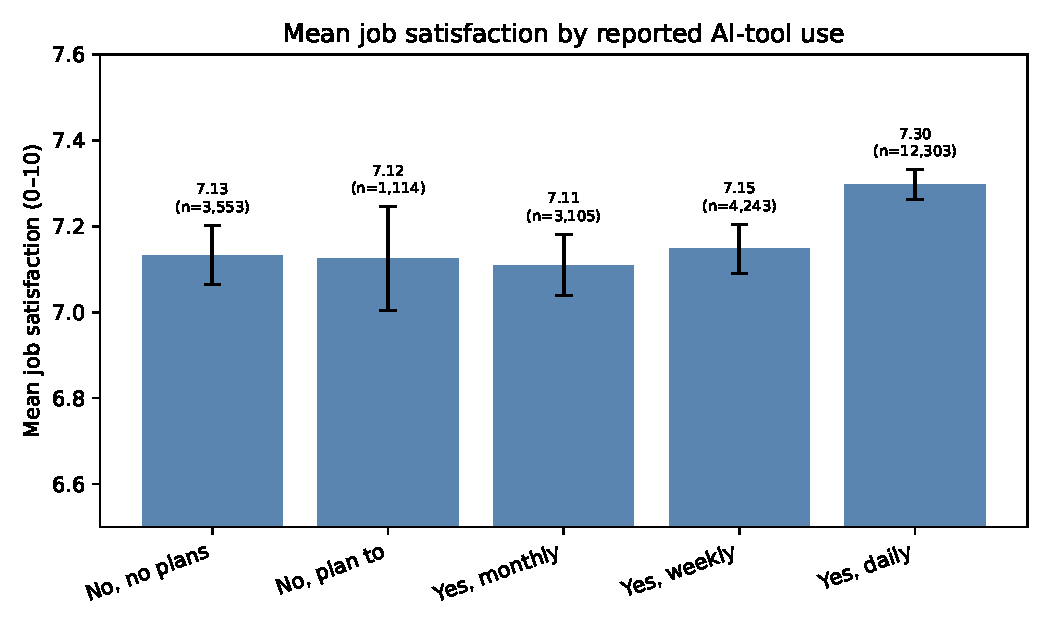
\includegraphics[width=0.8\linewidth]{figures/fig1_satisfaction_by_ai_use.pdf}
  \caption{Mean self-reported job satisfaction ($0$--$10$) by reported
  AI-tool use, among 24{,}318 professional developers in the analysis
  sample. Bars show category means; whiskers are $95\%$ confidence
  intervals; cell sizes are printed above each bar. The four non-daily
  categories cluster near $7.1$; daily users are slightly higher at
  $7.30$.}
  \label{fig:sat-by-ai}
\end{figure}

\begin{figure}[h]
  \centering
  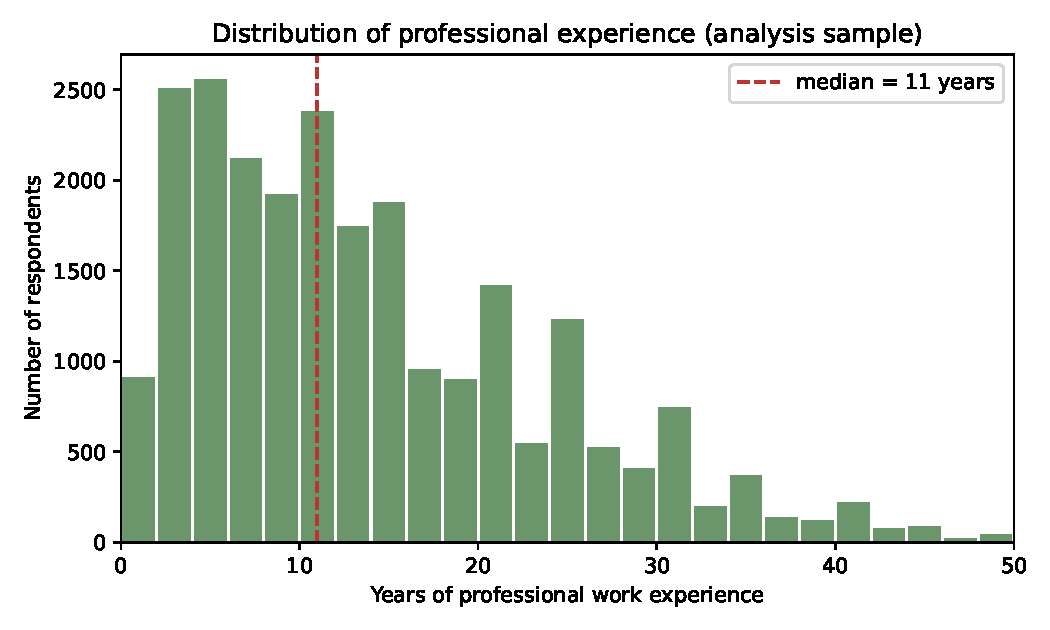
\includegraphics[width=0.8\linewidth]{figures/fig2_years_experience.pdf}
  \caption{Distribution of years of professional work experience among the
  24{,}318 professional developers in the analysis sample. The distribution
  is right-skewed with a median of $11$ years (dashed line); the long right
  tail reflects a minority of very experienced respondents.}
  \label{fig:years}
\end{figure}

\section{Limitations}
\label{sec:limitations}
The limitations are the most important part of this paper, because they,
not the coefficient, determine what may be concluded. The headline point is
simple: \emph{nothing here supports a causal interpretation.}

\textbf{Selection into the survey is not random.} The Stack Overflow survey
is a voluntary convenience sample recruited largely through Stack Overflow's
own audience. Developers who take the survey differ from those who do not,
and the differences plausibly relate to both AI-tool use and job
satisfaction. The sample is not representative of any defined population of
developers, so even the descriptive means generalise only with caution.

\textbf{AI-tool adoption is self-reported.} We observe what respondents say
about their AI-tool use, not their actual use. Self-reports may be coloured
by enthusiasm, social desirability, or differing interpretations of what
counts as ``using AI tools.''

\textbf{Job satisfaction is self-reported.} The outcome is a single
$0$--$10$ self-rating collected at one moment. It is subjective, sensitive
to mood and framing, and not anchored to any objective benchmark. Common
self-report method bias could inflate the association if the same
disposition pushes a respondent to report both higher tool use and higher
satisfaction.

\textbf{There is no instrument for AI-tool adoption.} We have no source of
variation in adoption that is plausibly unrelated to satisfaction except
through adoption. Without such an instrument (or an experiment), we cannot
separate any effect of the tools from selection into using them.

\textbf{The design is cross-sectional.} All variables are measured at once.
We cannot observe a developer's satisfaction before and after adopting AI
tools, so we cannot rule out reverse causation: more satisfied developers
may simply be more inclined to try new tools.

\textbf{Omitted variables are plausibly correlated with both sides.}
Developer ability, team culture, employer quality, compensation, and
autonomy are all things we do not adequately observe, and each could raise
both AI-tool adoption and job satisfaction. Our controls --- experience and
role --- absorb only a fraction of this, consistent with the model's very
low $R^2$. The adjusted coefficient should be read as ``the satisfaction
gap that remains after accounting for experience and role,'' not as an
effect net of confounding.

Finally, missingness is heavy and non-random: many respondents do not
answer the satisfaction item at all, and those who skip it may differ
systematically from those who answer. Our complete-case analysis ignores
this and could be biased as a result.

\section{Conclusion}
We document a small, statistically robust, positive cross-sectional
association between reported AI-tool adoption and reported job satisfaction
among professional developers in the Stack Overflow 2025 survey: roughly
$0.15$ points on a $0$--$10$ scale after adjusting for experience and role,
stable across specifications but explaining only about $2\%$ of the
variation in satisfaction. We did \emph{not} find, and did not attempt to
estimate, an effect of AI tools on satisfaction; the association is
consistent with selection, reverse causation, and omitted variables in
equal measure.

This paper is a teaching artefact for a seminar on AI for research. Its
purpose is to show the full loop --- from a public dataset to a short,
reproducible, honestly hedged write-up --- and to make visible where such
analyses are weakest: not in the arithmetic, which is easy, but in the
identification and the citations, which are not. Readers should take away
the workflow and the discipline of the limitations section, not the
coefficient.

\bibliographystyle{plainnat}
\bibliography{refs}

\end{document}
